\documentclass[]{article}
\usepackage{amsmath}
\usepackage{amsfonts}
\usepackage{amssymb}
\usepackage{graphicx}
\usepackage[margin=0.5in]{geometry}
\usepackage{float}
\usepackage{xcolor,cancel}
\setlength{\parindent}{0pt}
\usepackage{empheq}
\usepackage{mleftright}
\usepackage{blkarray}
\usepackage[normalem]{ulem}
\usepackage{xcolor}
\usepackage{esvect}

\definecolor{lightblue}{rgb}{0.68, 0.85, 0.9}
\newcommand\redsout{\bgroup\markoverwith{\textcolor{red}{\rule[1ex]{3pt}{0.5pt}}}\ULon}
%opening
\title{cart spring pendulum problem}
\author{Aravind Sundararajan}

\newcommand\hcancel[2][black]{\setbox0=\hbox{$#2$}%
	\rlap{\raisebox{.45\ht0}{\textcolor{#1}{\rule{\wd0}{1pt}}}}#2}

\begin{document}

\maketitle
\section{picture}
\begin{figure}[H]
	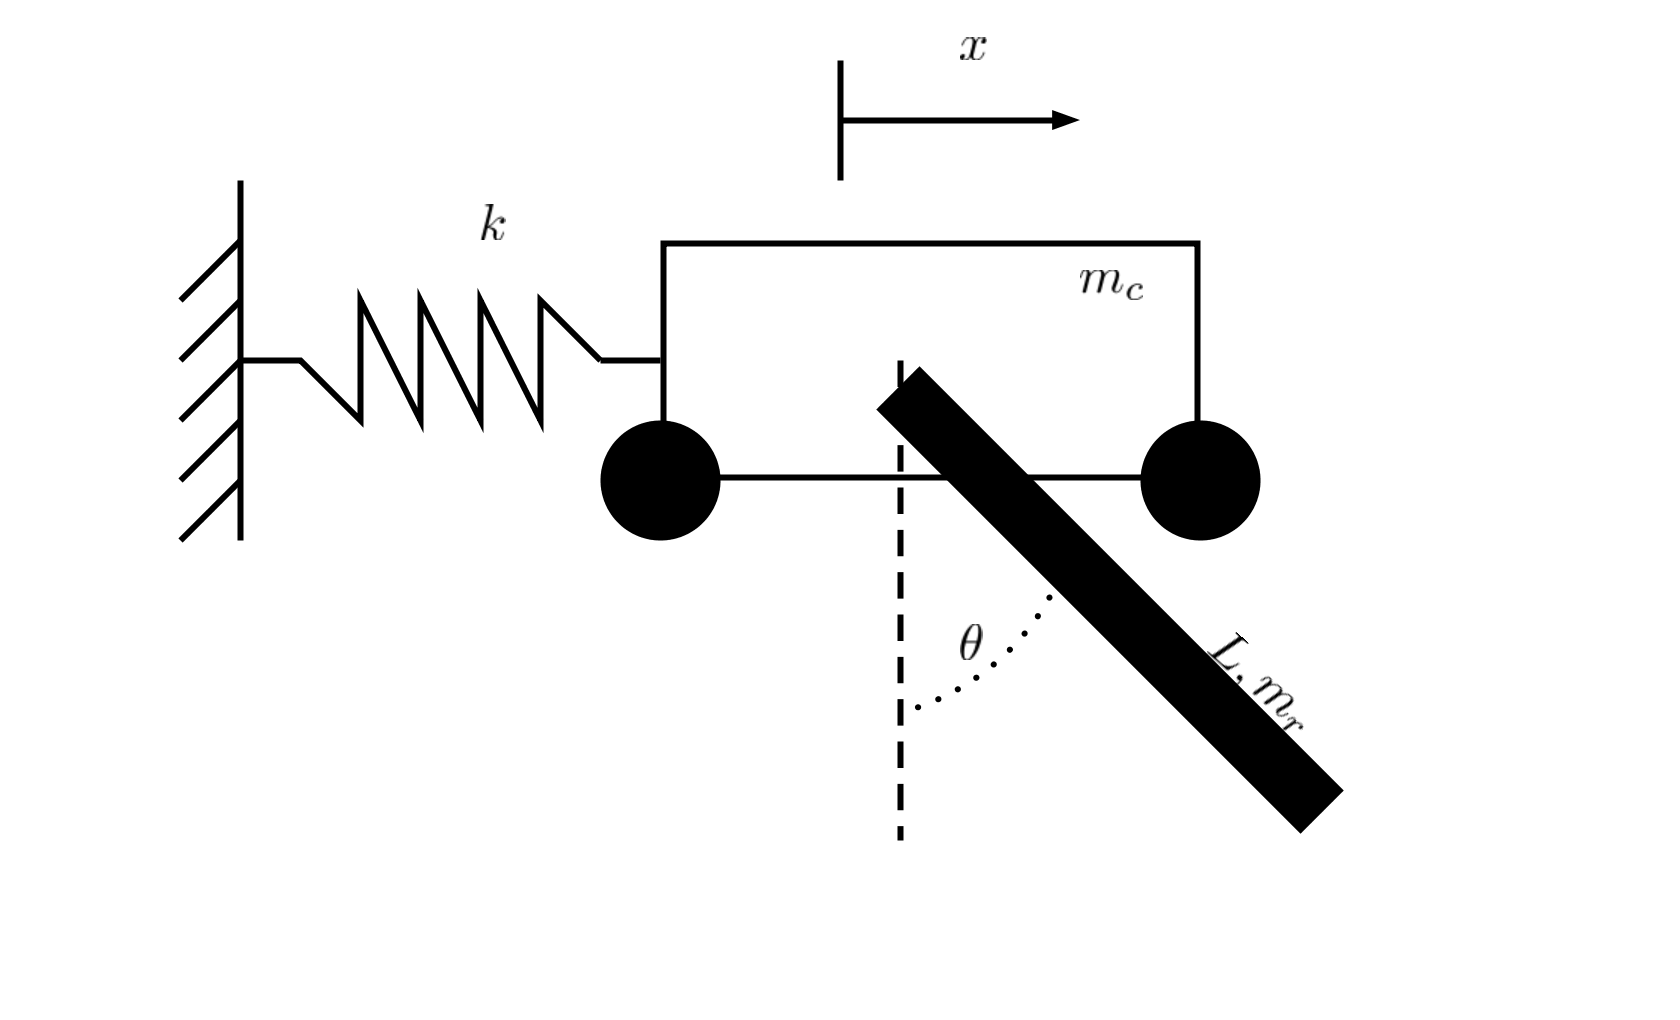
\includegraphics[width=.75\linewidth] {cart_problem.png}
\end{figure}
Also note that:

$k = 10 N/m$

$L = 0.5 m$

$m_c = 1 kg$

$m_r = 0.25 kg$

\newpage

\section{solve for EOM}
$$Y_G = \frac{L}{2}$$
$$I_G = \frac{1}{3} m L^2$$
$$r_G = (x + \frac{L}{2} s\theta) \vec{i} + (- \frac{1}{2} L c\theta) \vec{j}$$
$$\dot{r}_G = (\dot{x} + \frac{L}{2} c\theta \dot{\theta}) \vec{i} + (\frac{L}{2} s\theta \dot{\theta}) \vec{j}$$

note that : 

$T_{total} = T_{cart} + T_{rod}$

so we first find $T_{rod}$
$$T_{rod} = \frac{1}{2} m \dot{r} \cdot \dot{r} + \frac{1}{2} I_G \dot{\theta}^2$$
$$ \dot{r} \cdot \dot{r} = (\dot{x} + \frac{L}{2} c\theta \dot{\theta})(\dot{x} + \frac{L}{2} c\theta \dot{\theta}) + (\frac{L}{2} s\theta \dot{\theta})(\frac{L}{2} s\theta \dot{\theta})= \dot{x}^2 + Lc\theta\dot{x}\dot{\theta} + \frac{L^2}{4} c^2\theta \dot{\theta}^2  + \frac{L^2}{4} s^2\theta \dot{\theta}^2$$
$$ \dot{r} \cdot \dot{r} = \dot{x}^2 + Lc\theta\dot{x}\dot{\theta} + \frac{L^2}{4}\dot{\theta}^2$$
$$\frac{1}{2} I_G \dot{\theta}^2 = \frac{1}{2} (\frac{1}{3} m_r L^2) \dot{\theta}^2 = \frac{1}{6} m_r L^2 \dot{\theta}^2$$
$$T_{rod} = \frac{1}{2} m_r (\dot{x}^2 + Lc\theta\dot{x}\dot{\theta} + \frac{L^2}{4}\dot{\theta}^2 + \frac{L^2}{3}  \dot{\theta}^2)$$
$$T_{cart} = \frac{1}{2} m_c \dot{x}^2 $$
So we can solve for $T_{total}$
$$
T_{total} = T_{cart} + T_{rod} =\frac{1}{2} m_c \dot{x}^2 + \frac{1}{2} m_r (\dot{x}^2 + Lc\theta\dot{x}\dot{\theta} + \frac{7 L^2}{12}  \dot{\theta}^2) 
$$
Now we have to solve for $V$
$$V = \frac{1}{2} k x^2 + \frac{1}{2}m_r g L (1-c\theta)  $$
by lagrange's eqn, we have:

$$
\frac{d}{dt} (\frac{dT}{d\dot{q}_k}) - \frac{dT}{dq_k} + \frac{dV}{dq_k} = 0
$$
So, we need expressions for $\frac{dT}{dx}$, $\frac{dT}{d \dot{x}}$, $\frac{dV}{dx}$, $\frac{dT}{d\theta}$, $\frac{dT}{d \dot{\theta}}$, $\frac{dV}{d\theta}$ to construct our two EOM

$$\frac{dT}{dx} = 0$$
$$\frac{dT}{d \dot{x}} = (m_c+  m_r)\dot{x} +\frac{1}{2} m_r Lc\theta \dot{\theta}$$
$$\frac{dV}{dx} = kx$$
$$\frac{dT}{d\theta}  =-\frac{1}{2} m_r L \dot{\theta} \dot{x} s\theta$$
$$\frac{dT}{d \dot{\theta}}  =\frac{1}{2} m_r L \dot{x} c\theta + \frac{7}{12} m_r L^2 \dot{\theta}$$
$$\frac{dV}{d\theta}  =\frac{1}{2} m_r g L s\theta$$

\newpage

EOM1:
$$\frac{d}{dt} (\frac{dT}{d\dot{x}}) - \frac{dT}{dx} + \frac{dV}{dx} = 0$$
$$\frac{d}{dt} ((m_c+  m_r)\dot{x} +\frac{1}{2} m_r Lc\theta \dot{\theta}) + kx = 0$$
$$\boxed{(m_c+  m_r)\ddot{x} +(\frac{1}{2} m_r Lc\theta) \ddot{\theta} - \frac{1}{2} m_r Ls\theta \dot{\theta}^2}$$

EOM2:
$$\frac{d}{dt} (\frac{dT}{d\dot{\theta}}) - \frac{dT}{d\theta} + \frac{dV}{d\theta} = 0$$
$$\frac{d}{dt} (\frac{1}{2} m_r L \dot{x} c\theta + \frac{7}{12} m_r L^2 \dot{\theta})+\frac{1}{2} m_r L \dot{\theta} \dot{x} s\theta + \frac{1}{2} m_r g L s\theta= 0$$
$$\frac{1}{2} m_r L \ddot{x} c\theta - \frac{1}{2} m_r L \dot{x} \dot{\theta} s\theta + \frac{7}{12} m_r L^2 \ddot{\theta} +\frac{1}{2} m_r L \dot{\theta} \dot{x} s\theta + \frac{1}{2} m_r g L s\theta $$

$$
\frac{1}{2} m_r L \ddot{x} c\theta + \frac{7}{12} m_r L^2 \ddot{\theta} + \frac{1}{2} m_r g L s\theta  = 0
$$

$$
\boxed{\ddot{x} c\theta + \frac{7}{6} L \ddot{\theta} +  g s\theta  = 0}
$$

\end{document}
